\documentclass[conference]{IEEEtran}
\IEEEoverridecommandlockouts
\usepackage{listings}
\usepackage{xcolor}
\usepackage{hyperref}
\usepackage{amsthm}
\usepackage{pgfplots}
\usepackage{graphicx}
\graphicspath{ {./conference_041818/} }
\lstset { %
    language=C++,
    backgroundcolor=\color{black!5}, % set backgroundcolor
    basicstyle=\footnotesize,% basic font setting
}
%New colors defined below
\definecolor{codegreen}{rgb}{0,0.6,0}
\definecolor{codegray}{rgb}{0.5,0.5,0.5}
\definecolor{codepurple}{rgb}{0.58,0,0.82}
\definecolor{backcolour}{rgb}{0.95,0.95,0.92}

%Code listing style named "mystyle"
\lstdefinestyle{mystyle}{
  backgroundcolor=\color{backcolour},   commentstyle=\color{codegreen},
  keywordstyle=\color{magenta},
  numberstyle=\tiny\color{codegray},
  stringstyle=\color{codepurple},
  basicstyle=\ttfamily\footnotesize,
  breakatwhitespace=false,         
  breaklines=true,                 
  captionpos=b,                    
  keepspaces=true,                 
  numbers=left,                    
  numbersep=5pt,                  
  showspaces=false,                
  showstringspaces=false,
  showtabs=false,                  
  tabsize=2
}

%"mystyle" code listing set
\lstset{style=mystyle}
% The preceding line is only needed to identify funding in the first footnote. If that is unneeded, please comment it out.
\usepackage{cite}
\usepackage{amsmath,amssymb,amsfonts}
\usepackage{algorithmic}
\usepackage{graphicx}
\usepackage{textcomp}
\usepackage{xcolor}
\def\BibTeX{{\rm B\kern-.05em{\sc i\kern-.025em b}\kern-.08em
    T\kern-.1667em\lower.7ex\hbox{E}\kern-.125emX}}
\begin{document}

\title{DAA Assignment-01\\
}

\author{\IEEEauthorblockN{ Mohammad Monish }
\IEEEauthorblockA{\textit{IIB2019033} \\
}
\and
\IEEEauthorblockN{Sanket Kokude}
\IEEEauthorblockA{\textit{IIB2019034} \\
}
\and
\IEEEauthorblockN{Harshit Kumar}
\IEEEauthorblockA{\textit{IIB2019035} \\
}
}

\maketitle

\begin{abstract}
In this report we designed a Divide and Conquer algorithm using which we  will search for a given key in row wise and column wise sorted matrix .

\end{abstract}

\section{Introduction}
Given an $n$x$n$ matrix, where every row and column is sorted in increasing order. Given a key, we decide whether this key is in the matrix. Solved using divide and conquer algorithm.\\
A divide-and-conquer algorithm recursively breaks down a problem into two or more sub-problems of the same or related type, until these become simple enough to be solved directly. The solutions to the sub-problems are then combined to give a solution to the original problem.


\section{Algorithm Design}
Following is divide and conquer algorithm:
\begin{itemize}
\item If the key lesser than the minimum element or greater than the maximum element in the matrix return false
\item If the matrix contains only one element then check for key and return true or false accordingly
\item Find the middle element.
\item If middle element is same as key return true.
\item If key is greater than the middle  then check if element is present in present in lower submatrix or upper right submatrix, If found return true else return false
\item If the key is lesser than the middle element then check if the key is present in vertical submatrix on the left side of the middle element or in upper right submatrix .
\item If found return true else return false.
\end{itemize}

\section{Algorithm and illustration}
We are given a matrix and indices of the first and last element of the matrix.We check if the matrix contains only one element then we check whether the element is equal to key or not and return true or false accordingly else we define two pointers midRow and midColumn which will be the indices of the middle element.Now there can be three cases as follows :- \\  \\
i) If the Middle element is equal to the key then we just print the indices of the middle element and return true.\\ \\
ii) When the key is lesser than than the middle element ,we recursively search for the key in vertical sub-matrix on the left side of the middle element and sub-matrix on the up-right of the middle element.If the key is found we print the indices and return true else if the key is not present in any of the two sub-matrix we return false. \\ \\
iii) When the key is greater than the middle element ,we recursively search the key in horizontal sub-matrix down the middle element and the right-up sub-matrix .If the key is found we print the indices and return true else if the key is not present in any of the two sub-matrix we return false. \\ \\

Suppose we are Given a nxn matrix, where every row and column is sorted in  increasing  order.Given  a  key,  how  to  decide  whether this key is in the matrix,where n is 10 and key is 79. \\ \\

$$
\begin{bmatrix}
1 & 2 & 3 & 4 & 5 & 6 & 7 & 8 & 9 & 10 \\
11 & 12 & 13 & 14 & 15 & 16 & 17 & 18 & 19 & 20 \\
21 & 22 & 23 & 24 & 25 & 26 & 27 & 28 & 29 & 30 \\
31 & 32 & 33 & 34 & 35 & 36 & 37 & 38 & 39 & 40 \\
41 & 42 & 43 & 44 & 45 & 46 & 47 & 48 & 49 & 50 \\
51 & 52 & 53 & 54 & 55 & 56 & 57 & 58 & 59 & 60 \\
61 & 62 & 63 & 64 & 65 & 66 & 67 & 68 & 69 & 70 \\
71 & 72 & 73 & 74 & 75 & 76 & 77 & 78 & \color{red}79 & 80 \\
81 & 82 & 83 & 84 & 85 & 86 & 87 & 88 & 89 & 90 \\
91 & 92 & 93 & 94 & 95 & 96 & 97 & 98 & 99 & 100 \\ 
\end{bmatrix}
$$
\\

We will divide the the problem into a number of subproblems that are smaller instances of the same problem Conquer the subproblems by solving them recursively. If the subproblem sizes are
small enough, however, just solve the subproblems in a straightforward manner.
Combine the solutions to the subproblems into the solution for the original problem.
When the subproblems are large enough to solve recursively, we call that the recursive case. Once the subproblems become small enough that we no longer recurse,
we say that the recursion “bottoms out” and that we have gotten down to the base
case. Sometimes, in addition to subproblems that are smaller instances of the same
problem, we have to solve subproblems that are not quite the same as the original
problem. We consider solving such subproblems as part of the combine step
same problem. \\

$$
\begin{bmatrix}
51 & 52 & 53 & 54 & 55 & 56 & 57 & 58 & 59 & 60 \\ 
61 & 62 & 63 & 64 & 65 & 66 & 67 & 68 & 69 & 70 \\
71 & 72 & 73 & 74 & 75 & 76 & 77 & 78 & \color{red}79 & 80 \\
81 & 82 & 83 & 84 & 85 & 86 & 87 & 88 & 89 & 90 \\
91 & 92 & 93 & 94 & 95 & 96 & 97 & 98 & 99 & 100 \\ 
\quad
\end{bmatrix}
$$
$$
\begin{bmatrix}
56 & 57 & 58 & 59 & 60 \\
66 & 67 & 68 & 69 & 70 \\
76 & 77 & 78 & \color{red}79 & 80 \\
\quad
\end{bmatrix}
$$

$$
\begin{bmatrix}
76 & 77 & 78 & \color{red}79 & 80 \\
\end{bmatrix}
$$
$$
\begin{bmatrix}
\color{red}79 & 80 \\ 
\end{bmatrix} 
$$
$$
\begin{bmatrix}
\color{red}79 \\
\end{bmatrix}
$$


\section{Algorithm Analysis}
\textbf{Time complexity:}

At each recursion call we are dividing the problem of n*n into two sub-problems one of the size n/2*n/2 and the other sub-problem of size n*n/2 (or n/2* n).So for our analysis we can we can assume it to two matrices of size n/2*n/2,So we are making three recursive calls for sub-problem of size n/2*n/2 and performing some operation which will be of constant time.\\\\

$T(n) = T(n/2) + T(n/2) + T(n/2) + O(1)$ \\
$T(n) = 3T(n/2) + O(1)$ \\
$T(n) = O(n^{log_{2}3})$ \\
 

The solution of recurrence is $O(n^{1.58})$ using Master Method.\\
\\
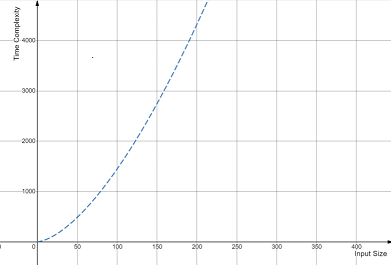
\includegraphics{Screenshot (257)}

\textbf{Space complexity:} O(n) \\


\section{Conclusion}
Finding the key with divide and conquer algorithm reduces the time complexity of searching ,which would be $O(n^{2})$ in case of linear searching.\\
Finally, Divide and Conquer algorithm works more efficiently.

 \section{References}
\color{blue}1.{\url{https://en.wikipedia.org/wiki/Divide-and-conquer_algorithm} }\\
2. {\url{https://www.geeksforgeeks.org/divide-and-conquer/}}\\
3. Cormen, Leiserson, Rivest, and Stein (2009). Introduction to Algorithms, 3rd edition.

\color{black}
\
\begin{titlepage}
    \begin{center}
        \Huge
        \section*{Appendix}
        \end{center}
         \textbf{Code for implementation of this paper is given below:}
\begin{lstlisting}[language=C++,caption=Code for this paper]
#include<bits/stdc++.h>
#include<vector>
using namespace std;

bool search(vector<vector<int> > &arr, int sRow, int eRow, int sColumn, int eColumn, int key) {
    // If the value of the key less than minimum value or greater than the maximum value in the matrix 
    // key cannot be in the matrix 
    if(key < arr[sRow][sColumn] or key >arr[eRow][eColumn])
    {
        return false;
    }
    // If this is a single element in the matrix 
    if (sRow == eRow and sColumn == eColumn) {
        if (key == arr[sRow][sColumn]) {
            cout << key << " Found at (" << sRow << "," << sColumn << ")" << endl;
            return true;
        } else {
            return false;
        }

    }
    int midRow = (sRow + eRow) / 2;
    int midColumn = (sColumn + eColumn) / 2;
    // If the middle element is equal to the key 
    if (arr[midRow][midColumn] == key) {
        cout << key << " Found at (" << midRow << "," << midColumn << ")" << endl;
        return true;
    } else if (key < arr[midRow][midColumn]) {
        bool a = false, b = false;
        if (midRow - 1 >= sRow) {
            a = search(arr, sRow, midRow - 1, midColumn, eColumn, key);
        }
        if (midColumn - 1 >= sColumn) {
            b = search(arr, sRow, eRow, sColumn, midColumn - 1, key);
        }

        return (a or b);
    } else // if key is greater than middle element 
    {
        bool a = false, b = false;
        //  If midColumn+1 does not exceed the number of Columns in the matrix 
        if (midColumn + 1 <= eColumn) {
            a = search(arr, sRow, midRow, midColumn + 1, eColumn, key);
        }
        // If midRow+1 does not exceed the number of row in the matrix 
        if (midRow + 1 <= eRow) {
            b = search(arr, midRow + 1, eRow, sColumn, eColumn, key);
        }
        // If the we can get key from any of the two calls return true
        return (a or b);
    }

}

int main() {
    
    int n=10; 
    //cout<<"Enter the value of n \n"; cin>>n
    vector<vector<int>> arr;
    arr.resize(n,vector<int>(n));

    int count = 1;
    for (int i = 0; i < n; i++) {
        for (int j = 0; j < n; j++) {
            //cin>>arr[i][j];
            arr[i][j] = count;
            count++;
        }
    }
    int key; 
    cout<<"Enter the value of key \n"; cin>>key;

    cout<<"The Given Matrix is\n";
    for (int i = 0; i < n; i++) {
        for (int j = 0; j < n; j++) {
            cout <<arr[i][j]<< " ";
            
        }
        cout << endl;
    }
    cout << endl;
    if (search(arr, 0, n - 1, 0, n - 1, key) == false) {
                cout << key << " Not Found\n";
    }
    return 0;
}
\end{lstlisting}
\end{titlepage}
\end{document}

